%!TEX root = index.tex
\chapter{Analises}
\label{cha:analises}

\section{Samsung}

A partir de conversas com Luís Guilherme Selber, responsável pela Operação do Laboratório Ocean, obtivemos a seguinte análise:

\begin{figure}[h]
\caption{Análise do Ocean - Samsung}
\centerline{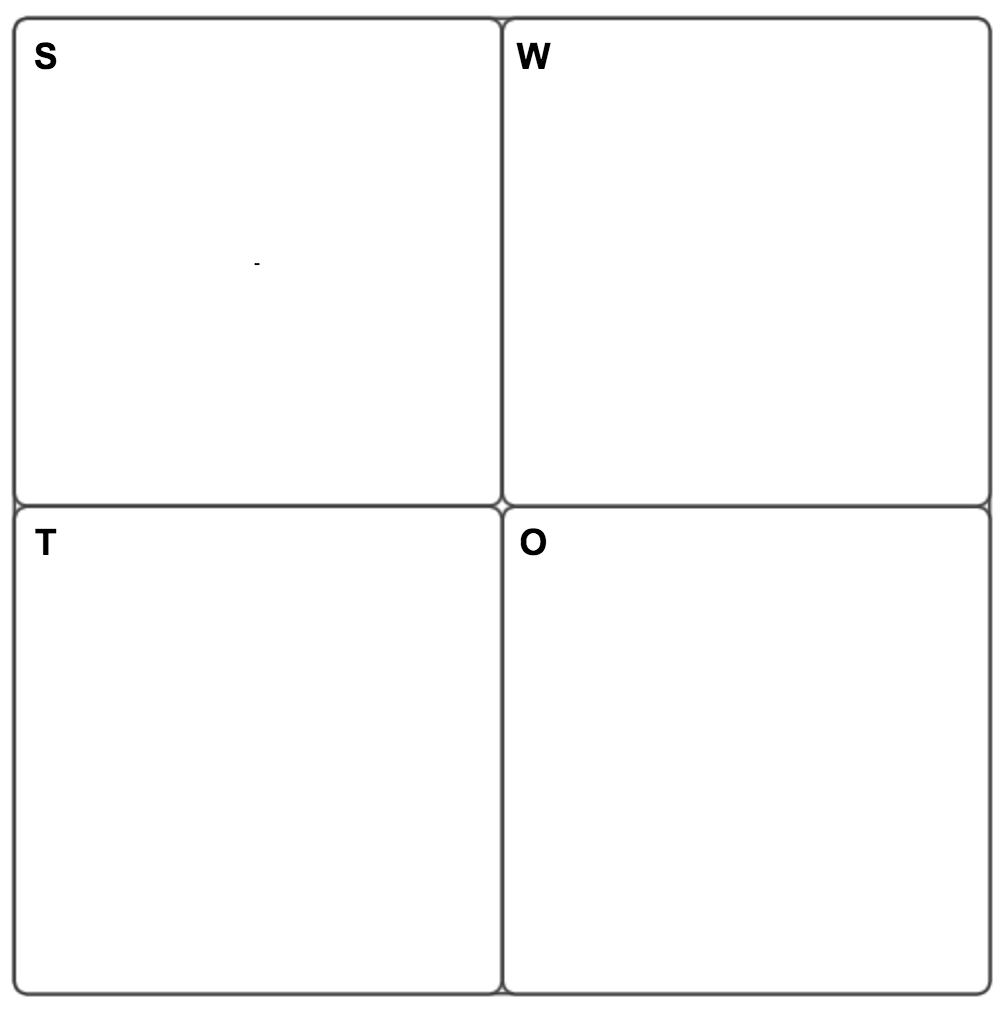
\includegraphics[scale=0.5]{img/generalswot}}
\label{fig:swotsamsung}
\caption* {Fonte: Elaborado pelo próprio autor}
\end{figure}

- Utilização do Espaço

1. O espaço é ocupado das 08 da manhã até as 22 da noite de segunda a quinta, fato que não acontecia na Faria Lima. Existia um papel da Samsung de sediar eventos próprios ou externos de forma a aumentar a utilização do espaço. 

Então mais pessoas utilizando desse espaço acaba divulgando mais o programa e os cursos oferecidos pelo laboratório, além de evitar com que a internet e equipamentos ficassem ociosos.

2. A USP é um ecossistema de parcerias com diversas empresas. O fato de estar dentro da Universidade por si só já coloca a Samsung em contato mais próximo com outras empresas, tendo provido reuniões com outras grandes empresas do mercado nacional.

3. Aumento da Demanda e de inscrições nos cursos intensivos, graças a participação de alunos e ex-alunos da própria universidade. 

- Cogestão Poli - Ocean

Situação atual: Ainda está baseado em reuniões pontuais e conversas de corredor, ainda em fase inicial, sem problemas da parte da samsung.
Futuro: Ter reuniões periódicas baseadas para definir melhor a utilização do espaço, projetos conjuntos...

Sobre a questão de utilização do espaço, a Samsung acredita que não haverá problema em relação a utilização do espaço, pois foi previamente alinhado as necessidades do uso do espaço pela Samsung e pela Universidade, sendo esse um ponto crítico para a parceria ter se estabelecido. Portas retrateis podem dividir o laboratório permitindo até 2 cursos em paralelo. 

\section{PRO}

\begin{figure}[h]
\caption{Análise do Ocean - PRO}
\centerline{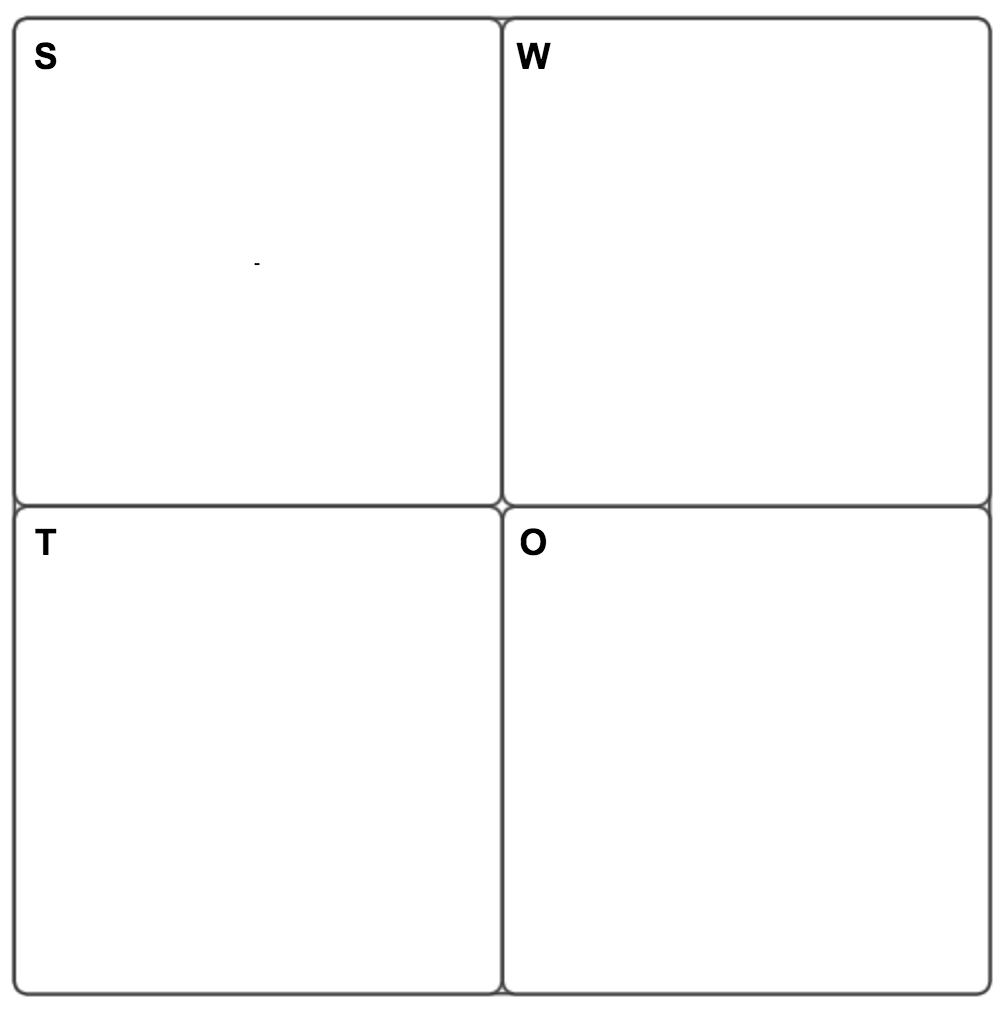
\includegraphics[scale=0.5]{img/generalswot}}
\label{fig:swotpro}
\caption* {Fonte: Elaborado pelo próprio autor}
\end{figure}

\section{Alunos}

\begin{figure}[H]
\caption{Análise do Ocean - Alunos}
\centerline{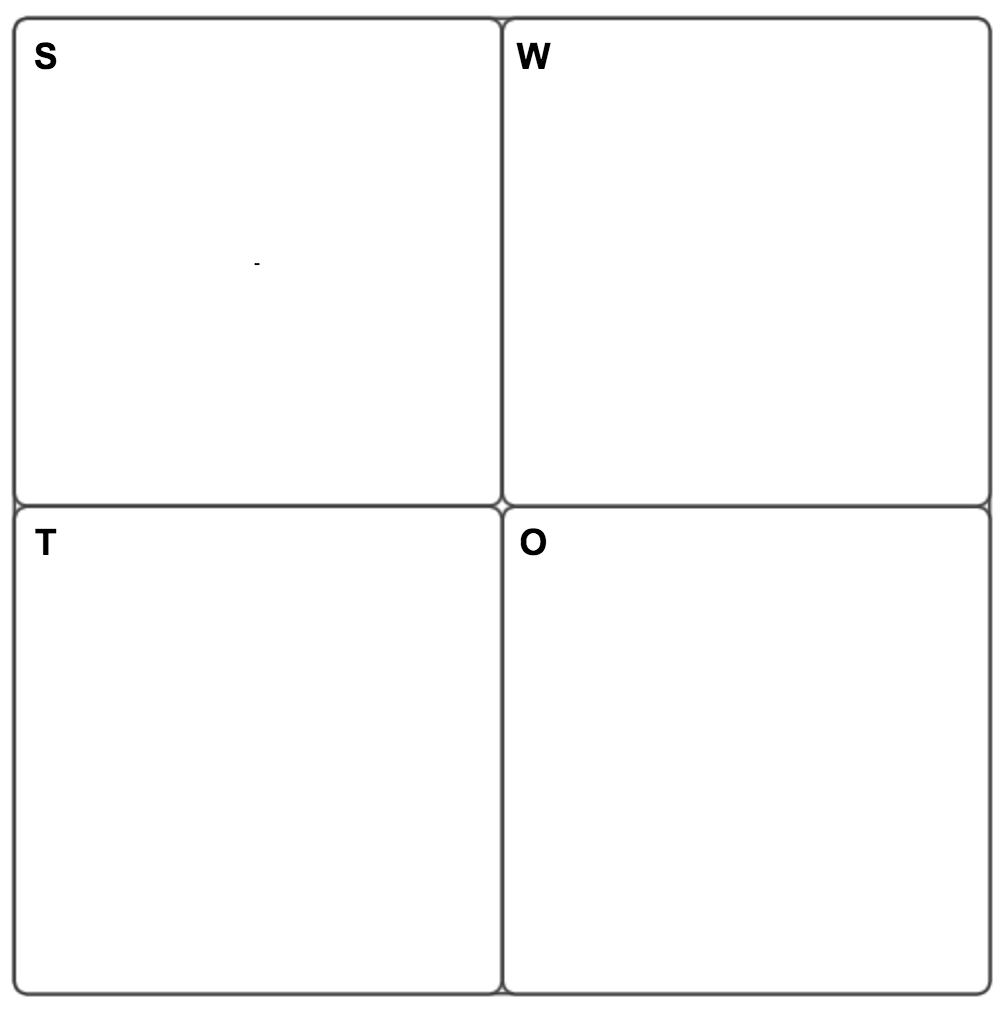
\includegraphics[scale=0.5]{img/generalswot}}
\label{fig:swotalunos}
\caption* {Fonte: Elaborado pelo próprio autor}
\end{figure}

\section{Usuários Externos}

\begin{figure}[h]
\caption{Análise do Ocean - Usuários Externos}
\centerline{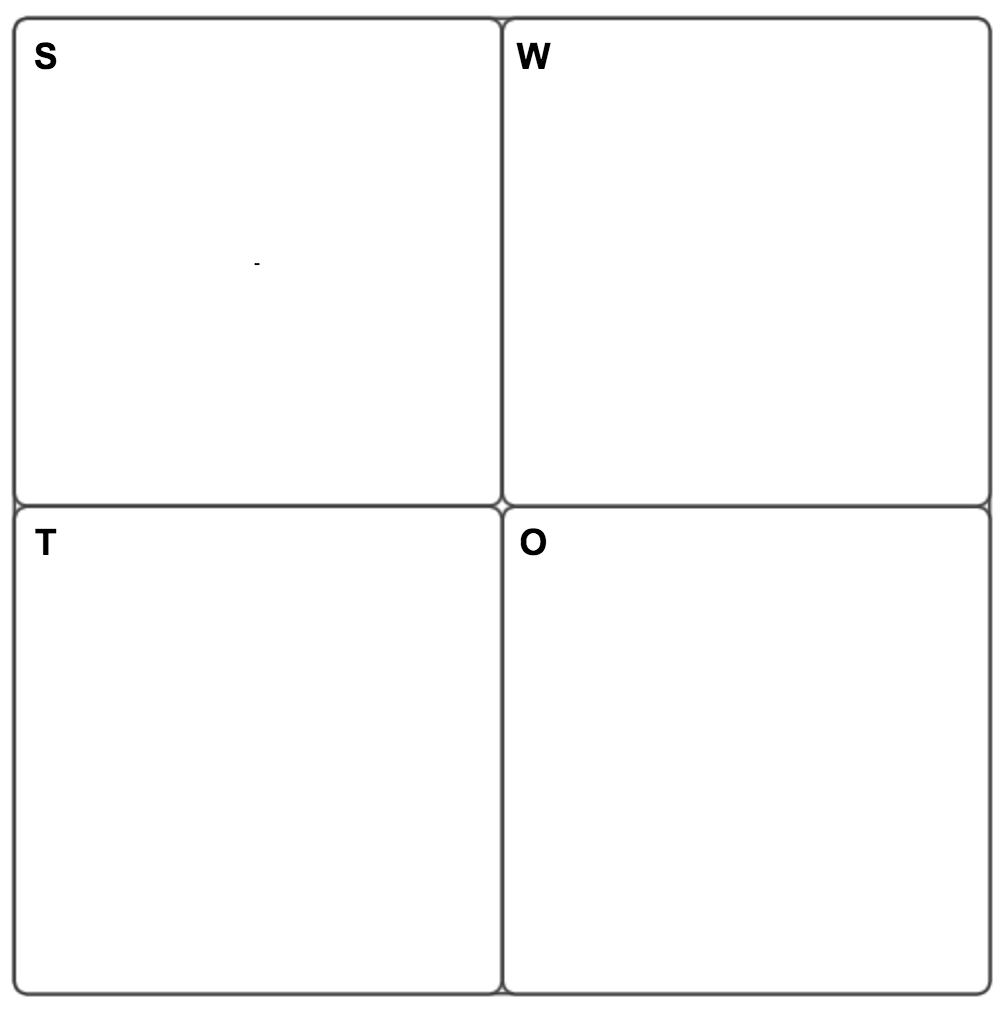
\includegraphics[scale=0.5]{img/generalswot}}
\label{fig:swotusuarios}
\caption* {Fonte: Elaborado pelo próprio autor}
\end{figure}